\documentclass[UTF8]{ctexbeamer}

\usetheme{Pittsburgh}
\usefonttheme[onlymath]{serif}

\usepackage{subfig}
\usepackage{multirow}
\usepackage{xcolor,colortbl}
\usepackage{listings}
\usepackage{amsmath}

% Solarized colors
\definecolor{sbase03}{HTML}{002B36}
\definecolor{sbase02}{HTML}{073642}
\definecolor{sbase01}{HTML}{586E75}
\definecolor{sbase00}{HTML}{657B83}
\definecolor{sbase0}{HTML}{839496}
\definecolor{sbase1}{HTML}{93A1A1}
\definecolor{sbase2}{HTML}{EEE8D5}
\definecolor{sbase3}{HTML}{FDF6E3}
\definecolor{syellow}{HTML}{B58900}
\definecolor{sorange}{HTML}{CB4B16}
\definecolor{sred}{HTML}{DC322F}
\definecolor{smagenta}{HTML}{D33682}
\definecolor{sviolet}{HTML}{6C71C4}
\definecolor{sblue}{HTML}{268BD2}
\definecolor{scyan}{HTML}{2AA198}
\definecolor{sgreen}{HTML}{859900}

\lstset{
    % How/what to match
    sensitive=true,
    % Border (above and below)
    frame=lines,
    % Extra margin on line (align with paragraph)
    xleftmargin=\parindent,
    % Put extra space under caption
    belowcaptionskip=1\baselineskip,
    % Colors
    backgroundcolor=\color{sbase3},
    basicstyle=\color{sbase00}\ttfamily,
    keywordstyle=\color{scyan},
    commentstyle=\color{sbase1},
    stringstyle=\color{sblue},
    numberstyle=\color{sviolet},
    identifierstyle=\color{sbase00},
    % Break long lines into multiple lines?
    breaklines=true,
    % Show a character for spaces?
    showstringspaces=false,
    tabsize=2
}


% Title
\title{第13章 连续模型的优化}
\author{韩建伟}
\institute{
  信息学院\\
  \texttt{hanjianwei@zjgsu.edu.cn}
}
\date{2019/12/18}

\begin{document}

% Title page
\begin{frame}[plain]
  \titlepage{}
\end{frame}

\begin{frame}{线性规划模型}
  \begin{block}{}
    \[ 
    \begin{array}{lcl}
      & \mbox{Opt}\ f(X) & \\
      \mbox{s.t.} & &  \\
      &
      g_i(X) \left\{
        \begin{array}{c}
          \ge\\
          \le
        \end{array}
      \right\} b_i& i \in I
    \end{array}
    \]
  \end{block}

  \begin{itemize}
  \item $f$是决策变量(即向量$X$的分量)的线性函数
  \item 约束函数$g_i$也必须是线性的
  \end{itemize}
  
\end{frame}

\begin{frame}{连续模型}
  \begin{block}{}
    \[ 
    \begin{array}{lcl}
      & \mbox{Opt}\ f(X) & \\
      \mbox{s.t.} & &  \\
      &
      g_i(X) = b_i& i \in I
    \end{array}
    \]
  \end{block}

  \begin{itemize}
  \item $f$连续但非线性
  \item 约束函数$g_i$也是非线性的, 但必须是等式约束
  \end{itemize}
  
\end{frame}

\begin{frame}{库存问题:送货费用和储存费用最小化}

  \begin{itemize}
  \item<1-> 公司希望利润最大化
  \item<2-> 假设短期内汽油的需求和价格是常数
  \item<3-> 最小化成本就能最大化利润
  \item<4-> 问题:每个加油站在保证持有足够多的汽油满足顾客需求的前提下,使每天平均的送
    货和库存持货成本最小 
  \end{itemize}

  \uncover<5-> {
    \[
      \text{日平均成本} = f(\text{存储费用}, \text{送货费用}, \text{产品需求率})
    \]
  }
  
\end{frame}

\begin{frame}{需求子模型}

  \begin{description}
  \item[存储费用] 假设单位产品的储存费用是常数
  \item[送货费用] 假设送货费用是常数,与送货量无关
  \item[需求] 假设需求量是函数
  \end{description}

  \begin{figure}
    \centering
    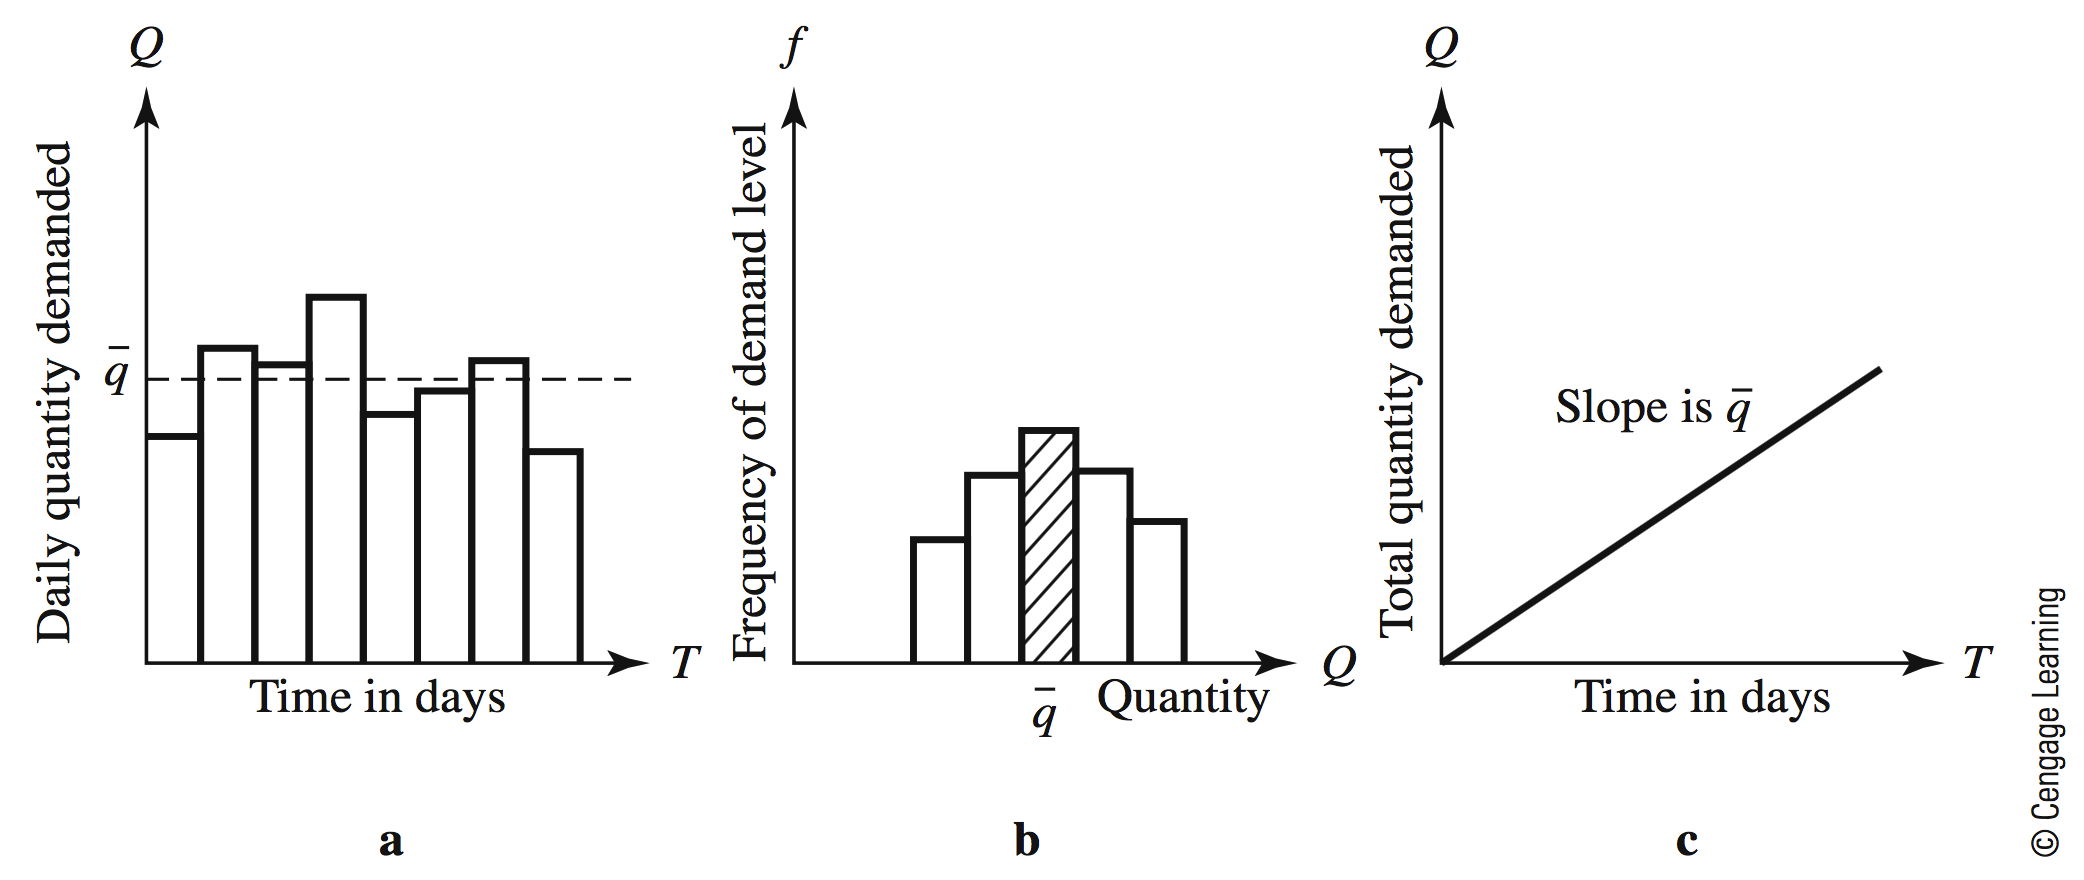
\includegraphics[width=.8\textwidth{}]{13_2.png}
  \end{figure}
  
\end{frame}

\begin{frame}{模型建立}

  \begin{itemize}
  \item $s$: 每加仑汽油储存一天的费用
  \item $d$: 每次送货的费用
  \item $r$: 需求率(加仑/天)
  \item $Q$: 每次订货的汽油量
  \item $t$: 时间(天)
  \end{itemize}

  \[
    \text{每个周期的费用} = d + s\frac{q}{2}t
  \]

  \begin{figure}
    \centering
    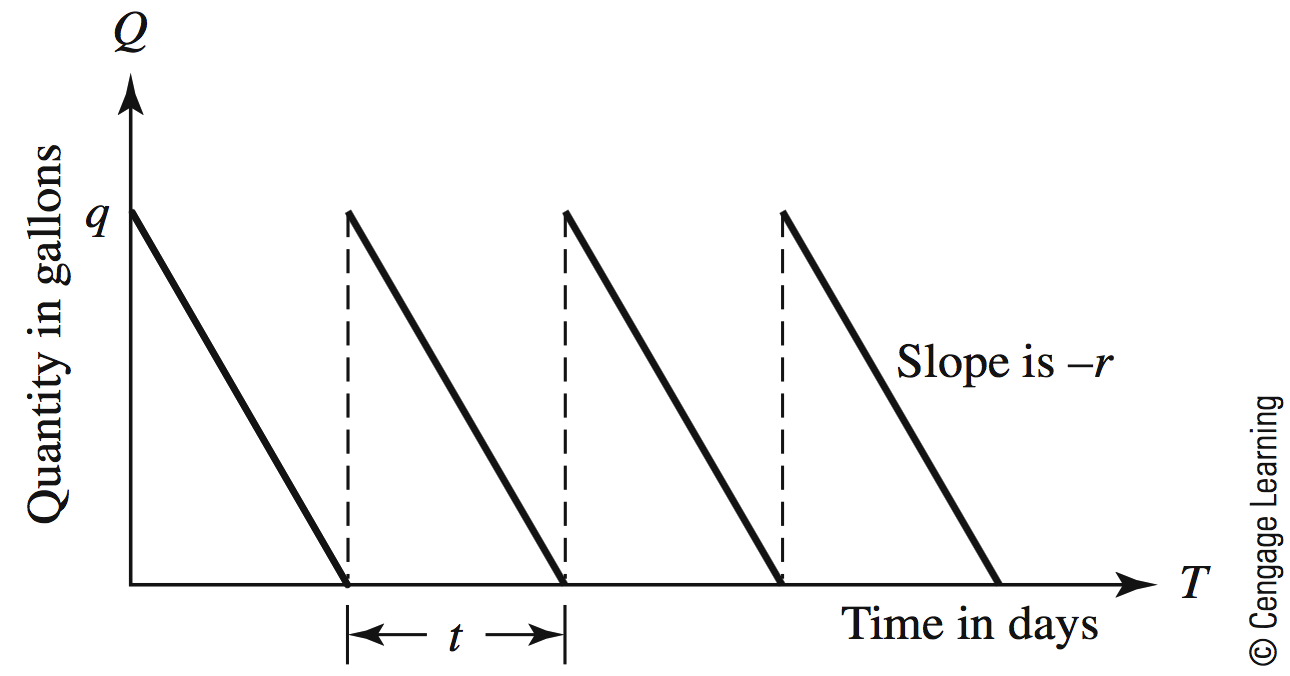
\includegraphics[width=.5\textwidth{}]{13_3.png}
  \end{figure}
  
\end{frame}

\begin{frame}{日均费用}
  \[
    c = \frac{d}{t} + \frac{s q}{2} = \frac{d}{t} + \frac{s r t}{2}
  \]

  \begin{figure}
    \centering
    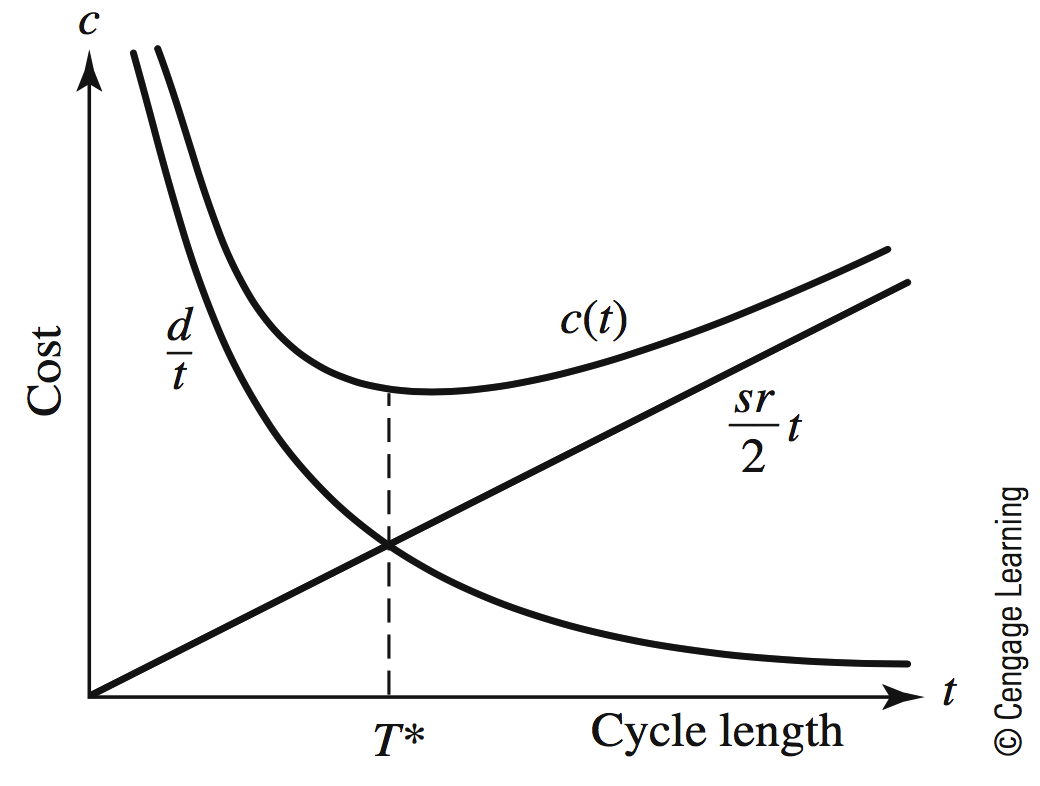
\includegraphics[width=.6\textwidth{}]{13_4.png}
  \end{figure}
\end{frame}

\begin{frame}{模型求解}

  \[
    c' = -\frac{d}{t^2} + \frac{s r}{2} = 0
  \]

  求得:

  \[
    T^\ast = \sqrt{ \frac{2 d}{s r} }
  \]

  \[
    c'' = \frac{2 d}{t^3}
  \]
  
\end{frame}

\begin{frame}{多变量函数的优化方法}

  \begin{gather*}
    P_1 = 3390 - 0.1 x_1 - 0.03 x_2\\
    P_2 = 3990 - 0.04 x_1 - 0.1 x_2\\
    R = P_1 x_1 + P_2 x_2\\
    C = 400000 + 1950 x_1 + 2250 x_2\\
    P = R - C\\
    x_1, x_2 \ge 0
  \end{gather*}
  
  
\end{frame}

\begin{frame}{多变量函数的求解}

  \[
    \frac{\partial P}{\partial x_1} = 0, \frac{\partial P}{\partial x_2} = 0
  \]

  \begin{figure}
    \centering
    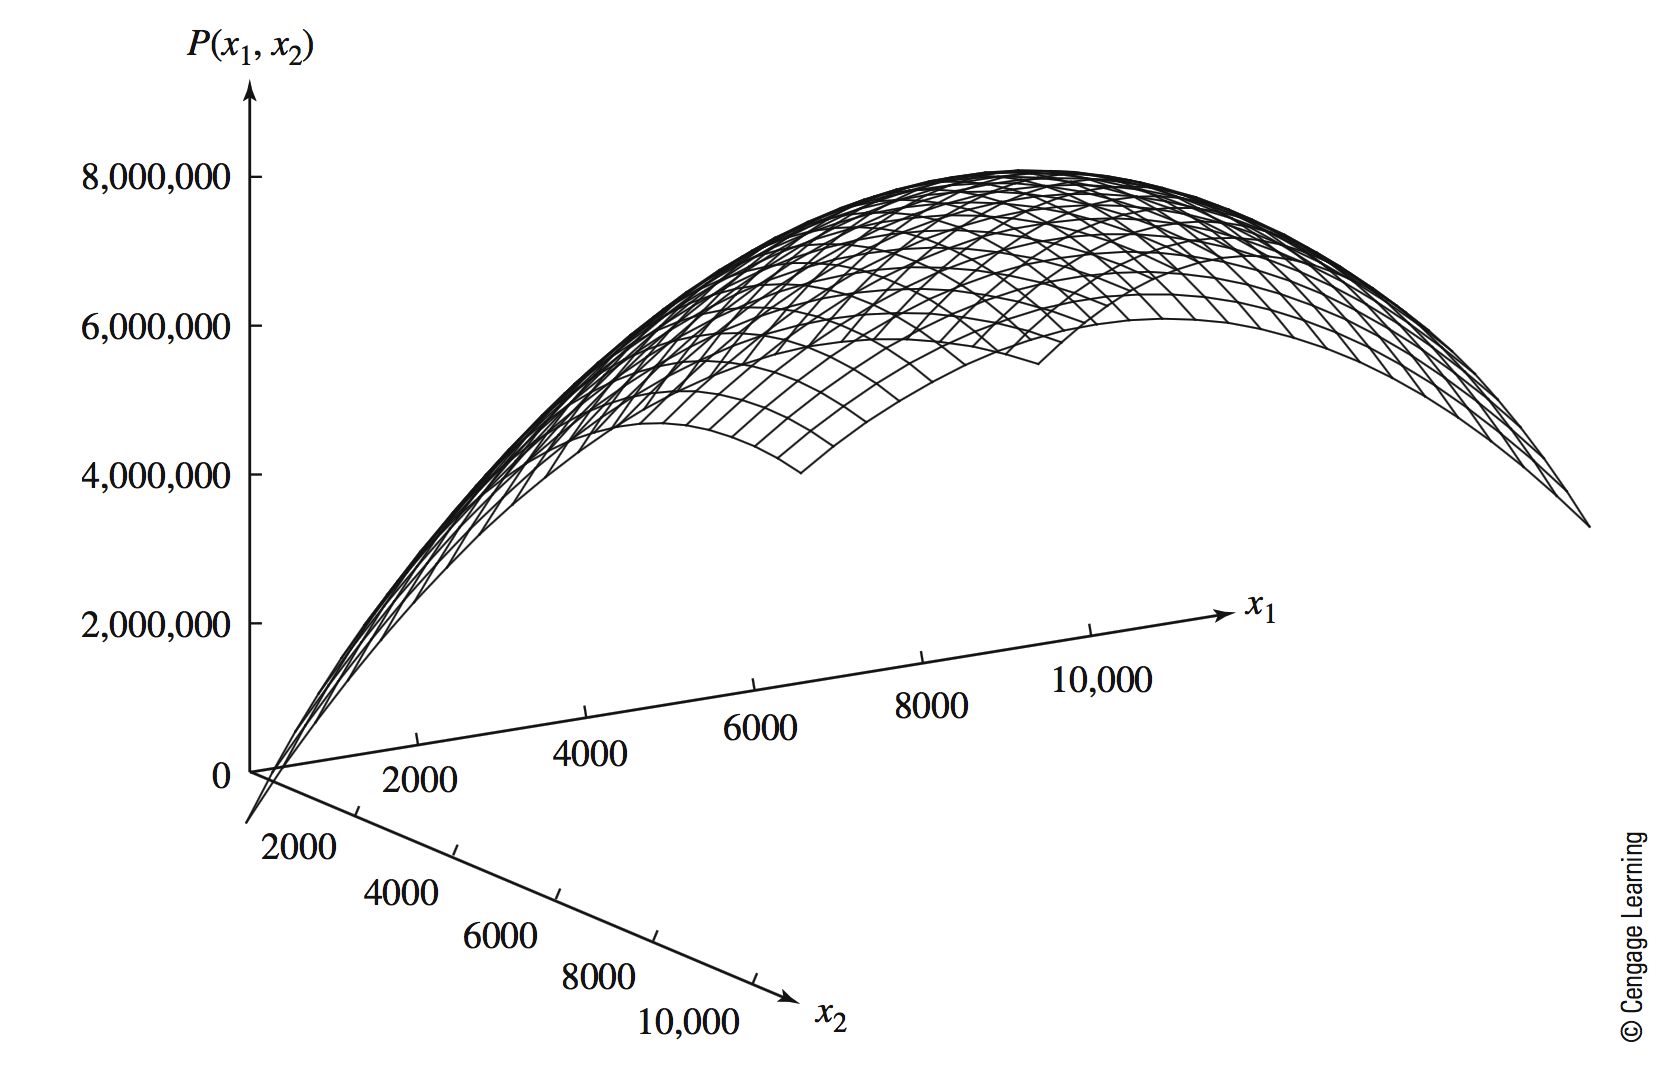
\includegraphics[width=.6\textwidth{}]{13_9.png}
  \end{figure}

  \begin{itemize}
  \item 最速下降法
  \end{itemize}
\end{frame}

\begin{frame}{连续约束优化}
  \begin{description}
  \item[问题] 在满足有限的存储空间约束的前提下,分配和维持足够的石油以满足需求,
    使总费用最小。
  \end{description}
  \begin{itemize}
  \item $x_i$: 储存第$i$类石油的数量
  \item $a_i$: 第$i$类石油的成本
  \item $b_i$: 单位时间取走第$i$类石油的速率
  \item $h_i$: 第$i$类石油单位时间的储存费
  \item $t_i$: 每单位第$i$类石油占用的储存空间
  \item $T$: 储存的总容量
  \end{itemize}
  
\end{frame}

\begin{frame}{优化模型}
  
  \begin{block}{}
    \[ 
    \begin{array}{lc}
      & \mbox{Min}\ f(x_1, x_2) = (\frac{a_1 b_1}{x_1} + \frac{h_1 x_1}{2}) + (\frac{a_2 b_2}{x_2} + \frac{h_2 x_2}{2}) \\
      \mbox{s.t.} &  \\
      &
      g(x_1, x_2) = t_1 x_1 + t_2 x_2 = T 
    \end{array}
    \]
  \end{block}

  \emph{拉格朗日乘子法}

  \[
    L(x_1, x_2, \lambda) = f(x_1, x_2) + \lambda (g(x_1, x_2) - T)
  \]

  令:

  \[
    \frac{\partial L}{\partial x_1} = \frac{\partial L}{\partial x_2} = \frac{\partial L}{\partial \lambda} = 0
  \]
  
\end{frame}
\end{document}

%%% Local Variables: 
%%% TeX-master: t
%%% TeX-engine: xetex
%%% End: 
